\newpage
\section{Stored Procedures, Triggers, and Functions}

\subsection{Stored Procedures for Insert, Update, and Delete}

This section presents the stored procedures used to perform insert, update, and delete operations on the \texttt{GAME} table. 
The \texttt{GAME} table was selected because it is one of the central entities of the Steam Store Management system. 
It stores digital game products that are later connected to developers, genres, DLCs, promotions, transactions, ownership records, and reviews.

The implementation includes three stored procedures: \texttt{sp\_InsertGame}, \texttt{sp\_UpdateGame}, and \texttt{sp\_DeleteGame}. 
These procedures centralize data modification logic and prevent invalid game data from being inserted, updated, or deleted directly.
\subsubsection{Selected Table and Operations}

The selected table for this part is \texttt{GAME}. 
This table stores the main product information of each game, including title, base price, release date, system requirements, and developer ID.

\begin{table}[H]
\centering
\caption{Stored procedures implemented for the \texttt{GAME} table}
\label{tab:game-crud-procedures}
\begin{tabular}{|l|p{9cm}|}
\hline
\textbf{Procedure} & \textbf{Purpose} \\ \hline
\texttt{sp\_InsertGame} & Inserts a new game into the \texttt{GAME} table after validating input values and developer existence. \\ \hline
\texttt{sp\_UpdateGame} & Updates an existing game after checking that the game exists and that the new values are valid. \\ \hline
\texttt{sp\_DeleteGame} & Deletes a game only if the game exists and is not already owned by players in their libraries. \\ \hline
\end{tabular}
\end{table}
\subsubsection{Procedure-level Validation}

The semantic constraints and business rules of the system were already discussed in Section 1.3. 
Therefore, this subsection only explains how the stored procedures apply relevant validation before modifying the \texttt{GAME} table.

The procedures validate required fields, data length, non-negative base price, reasonable release date, developer existence, duplicate game titles, and whether a game can be safely deleted. 
In particular, the delete procedure does not allow deleting a game that already exists in players' libraries, because this would break ownership records and affect historical user data.

When invalid input is detected, the procedures use \texttt{SIGNAL SQLSTATE '45000'} with specific error messages instead of generic error notifications.
\subsubsection{Full SQL Implementation}

The following SQL script shows the complete implementation of the three stored procedures (\texttt{sp\_InsertGame}, \texttt{sp\_UpdateGame}, and \texttt{sp\_DeleteGame}) used by the group for the \texttt{GAME} table.

\begin{lstlisting}[language=SQL, caption={Full SQL script for the insert, update, and delete stored procedures on the \texttt{GAME} table}, label={lst:game-crud-procedures}]
DELIMITER //

-- =============================================
-- 1. INSERT PROCEDURE
-- =============================================
CREATE PROCEDURE sp_InsertGame(
    IN p_title VARCHAR(100),
    IN p_base_price DECIMAL(10,2),
    IN p_release_date DATE,
    IN p_graphics VARCHAR(50),
    IN p_os VARCHAR(50),
    IN p_processor VARCHAR(50),
    IN p_memory VARCHAR(50),
    IN p_developer_id INT
)
BEGIN
    IF p_title IS NULL OR TRIM(p_title) = '' THEN
        SIGNAL SQLSTATE '45000' SET MESSAGE_TEXT = 'Error: Game title cannot be empty.';
    END IF;
    IF CHAR_LENGTH(p_title) > 100 THEN
        SIGNAL SQLSTATE '45000' SET MESSAGE_TEXT = 'Error: Title exceeds 100 characters.';
    END IF;
    IF CHAR_LENGTH(p_graphics) > 50 THEN
        SIGNAL SQLSTATE '45000' SET MESSAGE_TEXT = 'Error: System requirement [Graphics] fields cannot exceed 50 characters.';
    END IF;
    IF CHAR_LENGTH(p_os) > 50 THEN
        SIGNAL SQLSTATE '45000' SET MESSAGE_TEXT = 'Error: System requirement fields [OS] cannot exceed 50 characters.';
    END IF;
    IF CHAR_LENGTH(p_processor) > 50 THEN
        SIGNAL SQLSTATE '45000' SET MESSAGE_TEXT = 'Error: System requirement fields [Processor] cannot exceed 50 characters.';
    END IF;
    IF CHAR_LENGTH(p_memory) > 50 THEN
        SIGNAL SQLSTATE '45000' SET MESSAGE_TEXT = 'Error: System requirement fields [Memory] cannot exceed 50 characters.';
    END IF;
    IF p_base_price IS NULL THEN
        SIGNAL SQLSTATE '45000' SET MESSAGE_TEXT = 'Error: Base price cannot be empty.';
    END IF;
    IF p_base_price < 0 THEN
        SIGNAL SQLSTATE '45000' SET MESSAGE_TEXT = 'Error: Base price cannot be a negative value.';
    END IF;
    IF p_release_date > DATE_ADD(CURDATE(), INTERVAL 100 YEAR) THEN
        SIGNAL SQLSTATE '45000' SET MESSAGE_TEXT = 'Error: Release date is too far in the future.';
    END IF;
    IF p_release_date < '1950-01-01' THEN
        SIGNAL SQLSTATE '45000' SET MESSAGE_TEXT = 'Error: Release date is too far in the past.';
    END IF;
    IF p_developer_id IS NULL THEN
        SIGNAL SQLSTATE '45000' SET MESSAGE_TEXT = 'Error: Developer ID cannot be empty.';
    END IF;
    IF NOT EXISTS (SELECT 1 FROM `DEVELOPER` WHERE user_id = p_developer_id) THEN
        SIGNAL SQLSTATE '45000' SET MESSAGE_TEXT = 'Error: Developer ID does not exist.';
    END IF;
    IF EXISTS (SELECT 1 FROM `GAME` WHERE title = p_title) THEN
        SIGNAL SQLSTATE '45000' SET MESSAGE_TEXT = 'Error: A game with this title already exists.';
    END IF;
    INSERT INTO `GAME` (title, base_price, release_date, graphics, os, processor, memory, developer_id)
    VALUES (TRIM(p_title), p_base_price, p_release_date, p_graphics, p_os, p_processor, p_memory, p_developer_id);
    
    SELECT 'Success: Game added successfully.' AS Result;
END //
-- =============================================
-- 2. UPDATE PROCEDURE
-- =============================================
CREATE PROCEDURE sp_UpdateGame(
    IN p_game_id INT,
    IN p_title VARCHAR(100),
    IN p_base_price DECIMAL(10,2),
    IN p_release_date DATE,
    IN p_graphics VARCHAR(50),
    IN p_os VARCHAR(50),
    IN p_processor VARCHAR(50),
    IN p_memory VARCHAR(50)
)
BEGIN
    IF p_game_id IS NULL THEN
		SIGNAL SQLSTATE '45000' SET MESSAGE_TEXT = 'Error: Game ID cannot be empty.';
	END IF;
    IF NOT EXISTS (SELECT 1 FROM `GAME` WHERE game_id = p_game_id) THEN
        SIGNAL SQLSTATE '45000' SET MESSAGE_TEXT = 'Error: Cannot update. Game ID not found.';
    END IF;
    IF p_title IS NULL OR TRIM(p_title) = '' THEN
        SIGNAL SQLSTATE '45000' SET MESSAGE_TEXT = 'Error: Game title cannot be empty.';
    END IF;
    IF CHAR_LENGTH(p_title) > 100 THEN
        SIGNAL SQLSTATE '45000' SET MESSAGE_TEXT = 'Error: Title exceeds 100 characters.';
    END IF;
    IF CHAR_LENGTH(p_graphics) > 50 THEN
        SIGNAL SQLSTATE '45000' SET MESSAGE_TEXT = 'Error: System requirement [Graphics] fields cannot exceed 50 characters.';
    END IF;
    IF CHAR_LENGTH(p_os) > 50 THEN
        SIGNAL SQLSTATE '45000' SET MESSAGE_TEXT = 'Error: System requirement fields [OS] cannot exceed 50 characters.';
    END IF;
    IF CHAR_LENGTH(p_processor) > 50 THEN
        SIGNAL SQLSTATE '45000' SET MESSAGE_TEXT = 'Error: System requirement fields [Processor] cannot exceed 50 characters.';
    END IF;
    IF CHAR_LENGTH(p_memory) > 50 THEN
        SIGNAL SQLSTATE '45000' SET MESSAGE_TEXT = 'Error: System requirement fields [Memory] cannot exceed 50 characters.';
    END IF;
    IF p_base_price IS NULL THEN
        SIGNAL SQLSTATE '45000' SET MESSAGE_TEXT = 'Error: Base price cannot be empty.';
    END IF;
    IF p_base_price < 0 THEN
        SIGNAL SQLSTATE '45000' SET MESSAGE_TEXT = 'Error: Base price cannot be a negative value.';
    END IF;
    IF p_release_date > DATE_ADD(CURDATE(), INTERVAL 100 YEAR) THEN
        SIGNAL SQLSTATE '45000' SET MESSAGE_TEXT = 'Error: Release date is too far in the future.';
    END IF;
    IF p_release_date < '1950-01-01' THEN
        SIGNAL SQLSTATE '45000' SET MESSAGE_TEXT = 'Error: Release date is too far in the past.';
    END IF;
    IF EXISTS (SELECT 1 FROM `GAME` WHERE title = p_title AND game_id != p_game_id) THEN
        SIGNAL SQLSTATE '45000' SET MESSAGE_TEXT = 'Error: A game with this title already exists.';
    END IF;
    UPDATE `GAME`
    SET title = TRIM(p_title),
        base_price = p_base_price,
        release_date = p_release_date,
        graphics = p_graphics,
        os = p_os,
        processor = p_processor,
        memory = p_memory
    WHERE game_id = p_game_id;
    SELECT 'Success: Game updated successfully.' AS Result;
END //
-- =============================================
-- 3. DELETE PROCEDURE
-- =============================================
CREATE PROCEDURE sp_DeleteGame(
    IN p_game_id INT
)
BEGIN
	IF p_game_id IS NULL THEN
		SIGNAL SQLSTATE '45000' SET MESSAGE_TEXT = 'Error: Game ID cannot be empty.';
	END IF;
    IF NOT EXISTS (SELECT 1 FROM `GAME` WHERE game_id = p_game_id) THEN
        SIGNAL SQLSTATE '45000' SET MESSAGE_TEXT = 'Error: Deletion failed. Game ID does not exist.';
    END IF;
    IF EXISTS (SELECT 1 FROM `OWNS_LIBRARY` WHERE game_id = p_game_id) THEN
        SIGNAL SQLSTATE '45000' SET MESSAGE_TEXT = 'Error: Cannot delete game. It is already owned by players in their library.';
    END IF;
    DELETE FROM `GAME` WHERE game_id = p_game_id;
    SELECT 'Success: Game deleted successfully.' AS Result;
END //
DELIMITER ;
\end{lstlisting}
\subsubsection{Test Cases}

After creating the stored procedures, the following SQL statements were used to test the insert, update, and delete operations on the \texttt{GAME} table. 
A temporary game record was inserted first, then updated, and finally deleted. 
The variable \texttt{@test\_game\_id} was used to store the ID of the newly inserted game so that the update and delete procedures could be tested on the same record.

\begin{lstlisting}[language=SQL, caption={Test cases for \texttt{GAME} insert, update, and delete procedures}, label={lst:game-crud-test}]
USE steam_store;

-- Test 1: Insert a new game
CALL sp_InsertGame(
    'Test Game For Procedure',
    250000.00,
    '2026-05-01',
    'GTX 1050',
    'Windows 10',
    'Intel i5',
    '8GB RAM',
    6
);

-- Check inserted game
SELECT *
FROM `GAME`
WHERE title = 'Test Game For Procedure';

-- Save inserted game ID
SET @test_game_id = (
    SELECT game_id
    FROM `GAME`
    WHERE title = 'Test Game For Procedure'
    LIMIT 1
);

-- Test 2: Update the inserted game
CALL sp_UpdateGame(
    @test_game_id,
    'Updated Test Game For Procedure',
    300000.00,
    '2026-05-02',
    'GTX 1060',
    'Windows 11',
    'Intel i5',
    '8GB RAM'
);

-- Check updated game
SELECT *
FROM `GAME`
WHERE game_id = @test_game_id;

-- Test 3: Delete the inserted game
CALL sp_DeleteGame(@test_game_id);

-- Check deleted game
SELECT *
FROM `GAME`
WHERE game_id = @test_game_id;
\end{lstlisting}
\subsubsection{Execution Result}

The test results show that the three procedures worked correctly. 
First, \texttt{sp\_InsertGame} successfully inserted a new game into the \texttt{GAME} table. 
Then, \texttt{sp\_UpdateGame} updated the inserted game using the saved game ID. 
Finally, \texttt{sp\_DeleteGame} removed the test game from the table.

\begin{figure}[H]
    \centering
    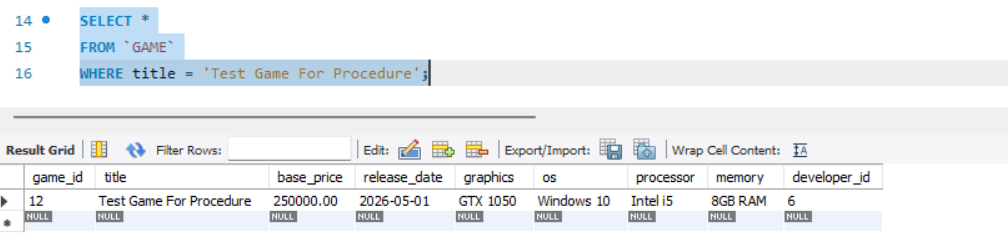
\includegraphics[width=0.9\linewidth]{graphics/game_insert_result.png}
    \caption{Result of inserting a new game using \texttt{sp\_InsertGame}}
    \label{fig:game-insert-result}
\end{figure}

\begin{figure}[H]
    \centering
    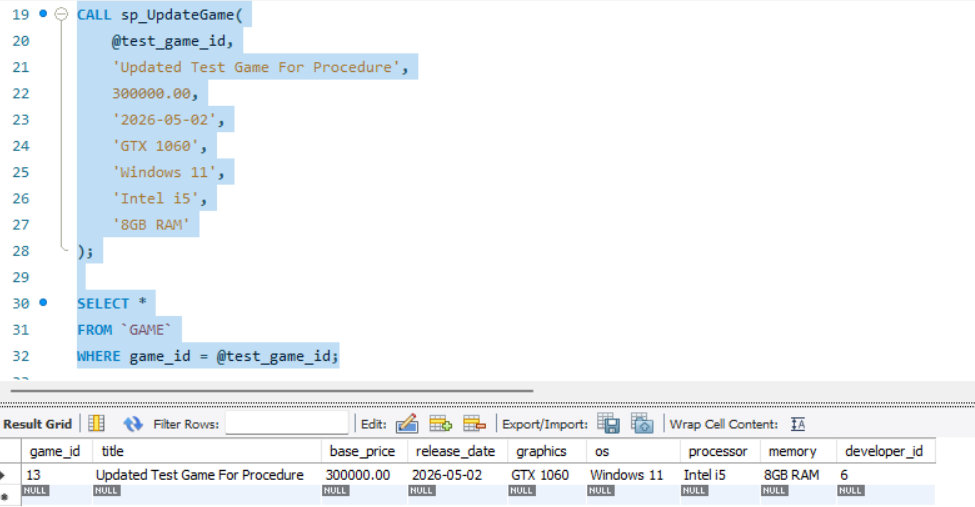
\includegraphics[width=0.9\linewidth]{graphics/game_update_result.png}
    \caption{Result of updating the inserted game using \texttt{sp\_UpdateGame}}
    \label{fig:game-update-result}
\end{figure}

\begin{figure}[H]
    \centering
    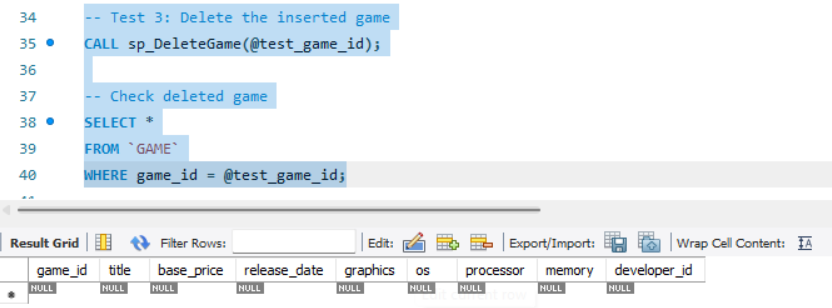
\includegraphics[width=0.9\linewidth]{graphics/game_delete_result.png}
    \caption{Result of deleting the test game using \texttt{sp\_DeleteGame}}
    \label{fig:game-delete-result}
\end{figure}